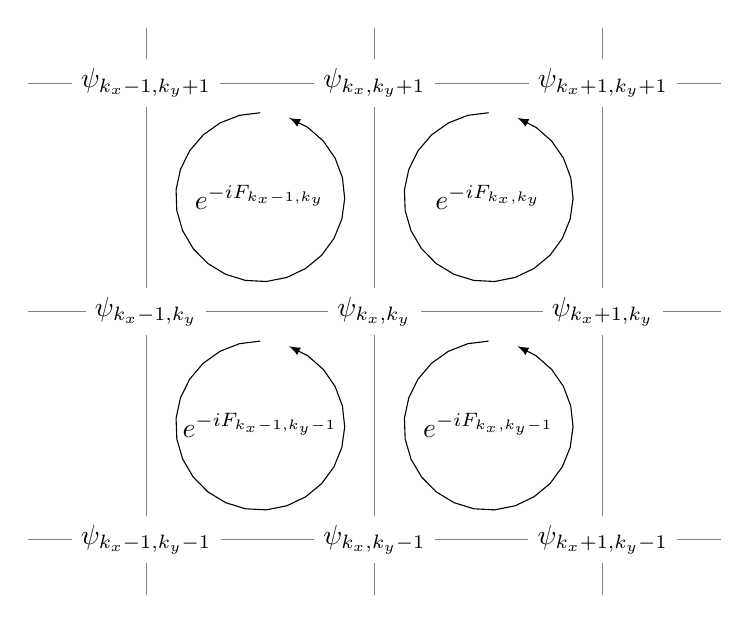
\begin{tikzpicture}

\def \gridsize{2.9}

\draw[step=\gridsize cm, help lines] (-\gridsize-1.5,-\gridsize-0.7) grid (\gridsize+1.5,\gridsize+0.7);
\draw node [fill= white] at (0,0) {$\ket{\psi_{k_x,k_y}}$};
\draw node [fill= white] at (\gridsize,0) {$\ket{\psi_{k_x+1,k_y}}$};
\draw node [fill= white] at (\gridsize,\gridsize) {$\ket{\psi_{k_x+1,k_y+1}}$};
\draw node [fill= white] at (0,\gridsize) {$\ket{\psi_{k_x,k_y+1}}$};
\draw node [fill= white] at (-\gridsize,0) {$\ket{\psi_{k_x-1,k_y}}$};
\draw node [fill= white] at (0,-\gridsize) {$\ket{\psi_{k_x,k_y-1}}$};
\draw node [fill= white] at (-\gridsize,-\gridsize) {$\ket{\psi_{k_x-1,k_y-1}}$};
\draw node [fill= white] at (\gridsize,-\gridsize) {$\ket{\psi_{k_x+1,k_y-1}}$};
\draw node [fill= white] at (-\gridsize,\gridsize) {$\ket{\psi_{k_x-1,k_y+1}}$};

\draw [-latex, domain = 0:340] plot ({0.37 *\gridsize* cos (\x + 90) + 0.5 * \gridsize }, {0.37 *\gridsize* sin (\x + 90) + 0.5 *\gridsize });
\draw [-latex, domain = 0:340] plot ({0.37 *\gridsize* cos (\x + 90) - 0.5 * \gridsize }, {0.37 *\gridsize* sin (\x + 90) + 0.5 *\gridsize });
\draw [-latex, domain = 0:340] plot ({0.37 *\gridsize* cos (\x + 90) + 0.5 * \gridsize }, {0.37 *\gridsize* sin (\x + 90) - 0.5 *\gridsize });
\draw [-latex, domain = 0:340] plot ({0.37 *\gridsize* cos (\x + 90) - 0.5 * \gridsize }, {0.37 *\gridsize* sin (\x + 90) - 0.5 *\gridsize });

\draw node at (0.5*\gridsize, 0.5*\gridsize) {$e^{-i F_{k_x,k_y}}$};
\draw node at (0.5*\gridsize, -0.5*\gridsize) {$e^{-i F_{k_x,k_y-1}}$};
\draw node at (-0.5*\gridsize, 0.5*\gridsize) {$e^{-i F_{k_x-1,k_y}}$};
\draw node at (-0.5*\gridsize, -0.5*\gridsize) {$e^{-i F_{k_x-1,k_y-1}}$};

\end{tikzpicture}